\chapter{Diseño del sistema}

 {\huge se utiliza la palabra barrera para hablar de los sensores SL y SL mini, aun no encuentro una palabra mejor para definirlas sin hacer referencia a eso}

En este capítulo se muestra el desarrollo general del sistema, comenzando por una vision superficial del sistema hasta obtener la versión final del sistema, la implementación del mismo se hará en los capítulos siguientes. [puede ser que se incluya una version final del sistema en una figura]
\section{Descripción general del sistema}

El requisito fundamental de este trabajo fue poder controlar el sistema de entrada y salida de vehiculos de al menos un resinto. Por lo que nos enfocaremos en comprender como funciona el sistema para el caso de un solo lugar. Adicionalmente existen otros requisitos preestablecidos, como:

\begin{itemize}
    \item Controlar el tiempo que el vehículo estuvo en el establecimiento.
    \item Que la entrada y salida sea automatica basada en la patente.
\end{itemize}


\begin{figure}
    \centering
    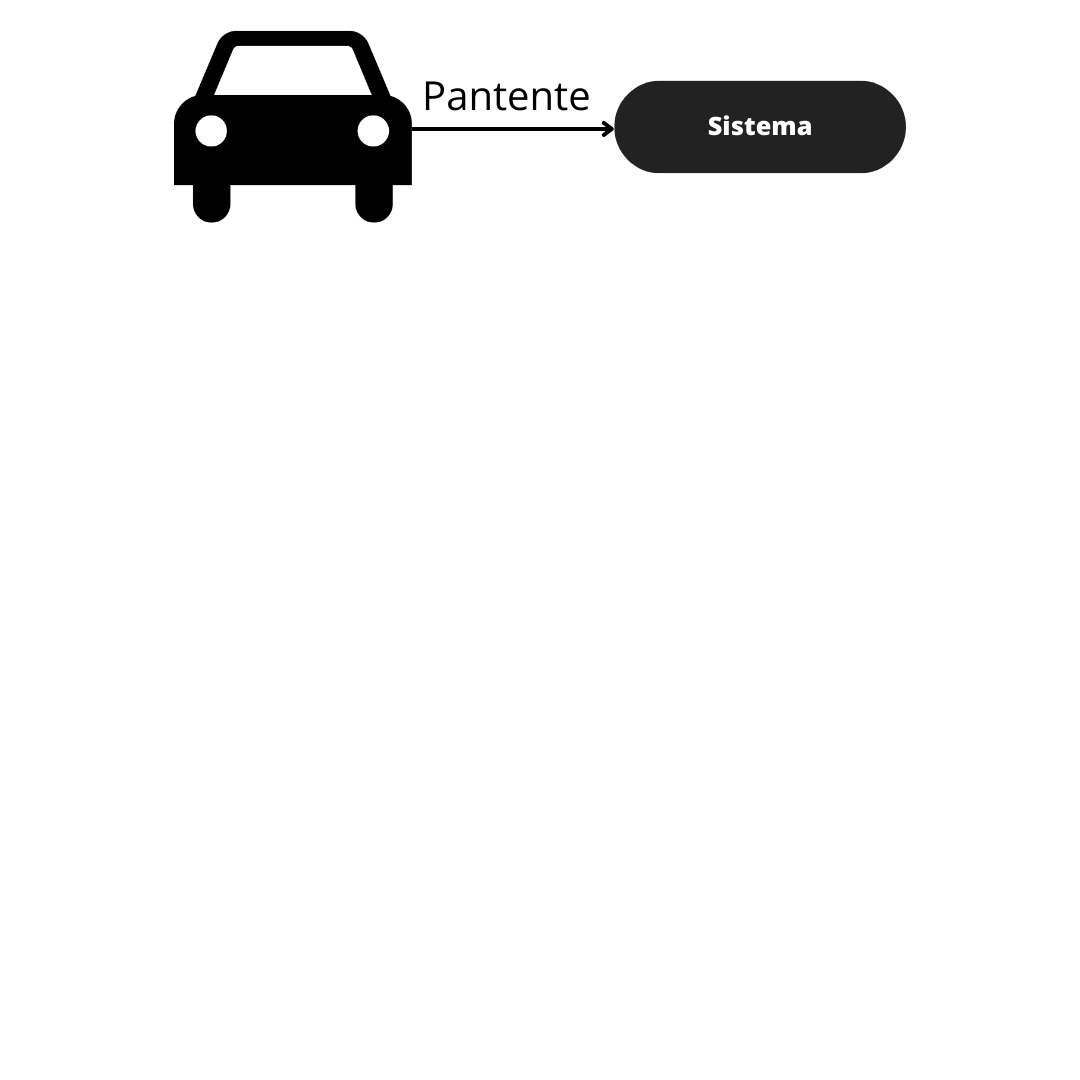
\includegraphics[width=.8\textwidth]{imgs/sistema-base.png}
    \caption{Versión inicial del sistema}
    \label{fig:sistema-base}
\end{figure}

De estos requisitos se desprende la forma más general del sistema, la cual cuenta con sistema que detecte los caracteres del vehículo, le permita el acceso o el egreso del establecimiento al vehículo y basado en la hora de entra y salida calcule el tiempo que estuvo el vehículo Fig. \ref{fig:sistema-base}.


Pensando en parques de estacionamiento, como los de los supermecados, es usual encontrarse que tiene entradas y salidas diferenciadas, es por ello que se decidio diferenciar la existencia de barreras que actuaran como entrada ó salida.

Otra problematica a la hora de pensar en un sistema automatico, es ¿Comó podemos detectar la patente? la respuesta, aunque simple muy utilizada, es utilizar una cámara para capturar un foto del vehículo. Un inconveniente es cúando sacar la foto, es por ello que se agregó un sensor para medir distancia, y evitar un período de muestreo estatico. De esta manera obtenemos la versión general del sistema Fig. \ref{fig:sistema-completa}.

\begin{figure}
    \centering
    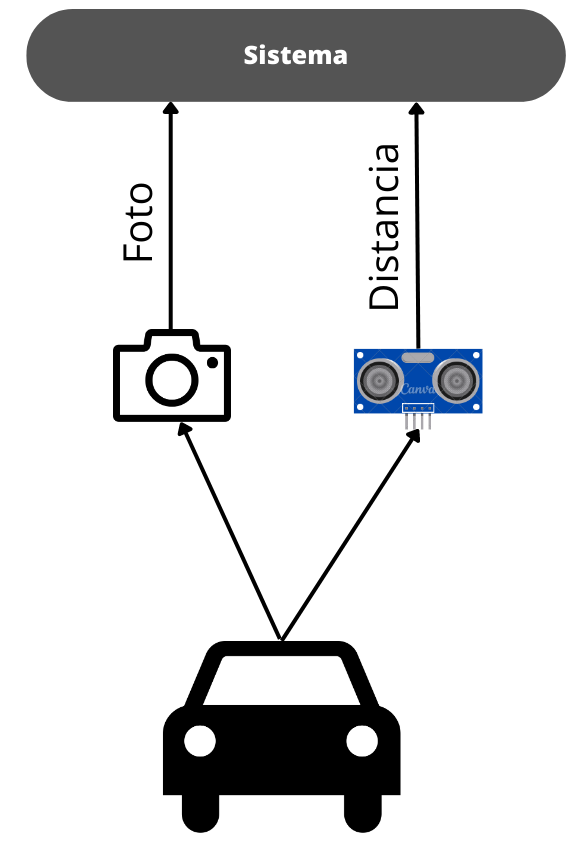
\includegraphics[width=.8\textwidth]{imgs/sistema-con-sensor.png}
    \caption{Sistema con sensor de distancia y camara}
    \label{fig:sistema-completa}
\end{figure}

\section{Los algoritmos de entrada y salida}

Una vez establecido nuestro sistema, obtenemos dos algoritmos muy similares, uno para la entrada del vehículo y otro para la salida. Es por ello que comenzaremos describiendo el algoritmo de entrada y luego pasaremos al algoritmo de salida.

\subsection{Algoritmo de entrada}

La toma de una muestras, es decir, una fotografía, se da cuando el sistema detecta que tiene un objeto a menos de $X$cm. Luego, se procesa la imagen, para obtener la patente en formato de texto, en caso de encontrar una patente, se almacena la fecha, junto con la patente y la fotografía Fig. \ref{fig:flujo-entrada}.

\begin{figure}
    \centering
    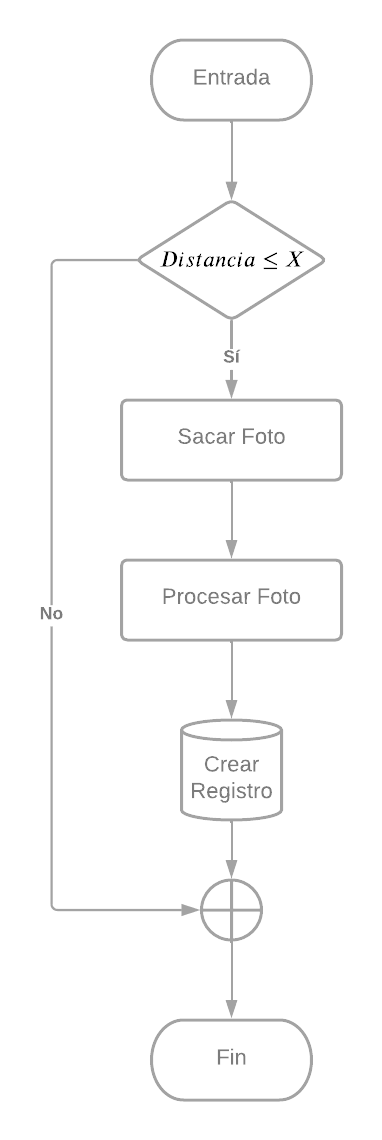
\includegraphics[width=.5\textwidth]{imgs/flujo-entrada.png}
    \caption{Diagrama de flujo para la entrada}
    \label{fig:flujo-entrada}
\end{figure}

\subsection{Algoritmo de salida}

El algoritmo de salida es identico, en la toma de muestra, pero antes de guardar la información de salida (foto y fecha), se verifica que exista un registro de entrada correspondiente y se actualiza el mismo Fig. \ref{fig:flujo-salida}.

\begin{figure}
    \centering
    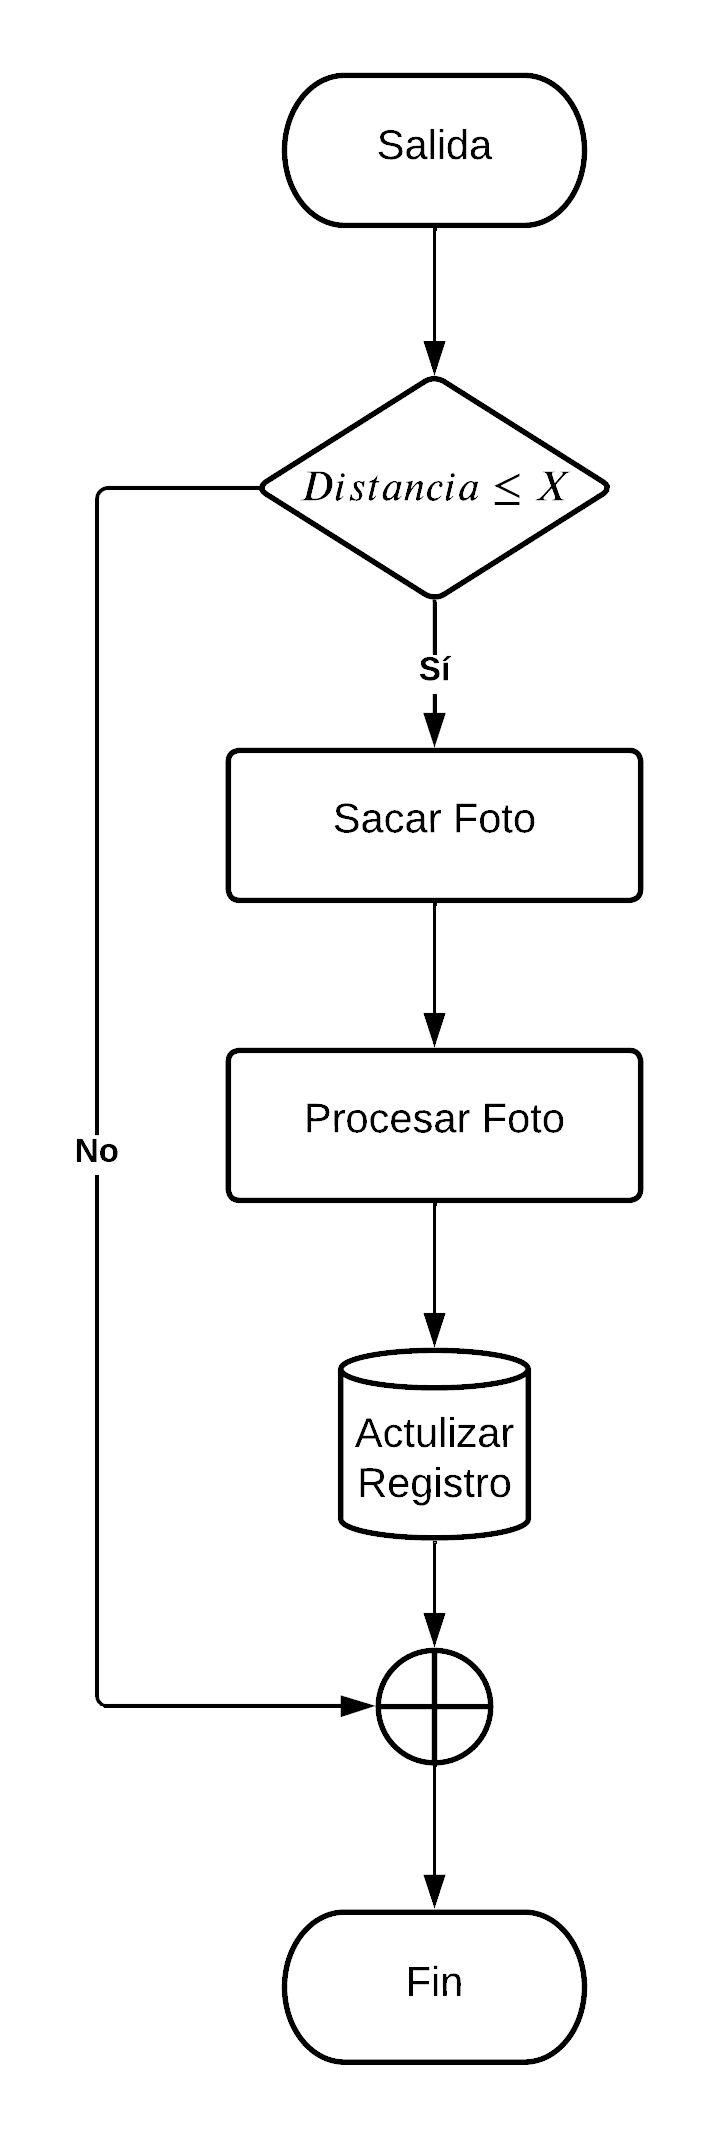
\includegraphics[width=.5\textwidth]{imgs/flujo-salida.png}
    \caption{Diagrama de flujo para la salida}
    \label{fig:flujo-salida}
\end{figure}

\subsection{El problema de multiples resintos}

Ambos algoritmo poseen un pequeño incoveniente a la hora de extender el proyecto en más de un resinto. Es por ello que cada barrera se vincula a un lugar, y los registros se buscan y actualizan en función del lugar que tiene la asignado cada barrera.
\section{Partes del sistema}

 {\huge quizas tengamos que agregar una seccion antes con la teoria de protocolo HTTP}

Una vez diseñado y comprendido como esta compuesto el sistema a grandes razgos, es importante entender las partes del mismo y lograr diferencias que parte del algortimo se ejecutara en la barrera y cual en el servidor. [agregar diagrama de la separación del sistema según server/barrera usar la SL como barrera]. Es importante destacar que la comunicación entre el servidor y las barreras se dará por 2 protocolos (HTTP y MQTT).

El envío de registros, tanto entrada como salida, es mediante HTTP, por otro lado las configuraciones de las barreras se hacen mendiante MQTT, lo que permite que el servidor envie los cambios de forma automatica, sin que la barrera tenga que realizar una petición HTTP cada cierto tiempo.

El esquema del sistema final, contemplando las barreras y el servidor se puede observar en ... [agregar diagrama final del sistema].

Esta versión del sistema ira desarrollando en los capítulos siguientes, yendo desde la transformación de foto a patente, la comunicación entre las diferentes partes del sistema, y otros detalles de implementación del sistema.